% Created by tikzDevice version 0.12.6 on 2024-02-29 10:34:55
% !TEX encoding = UTF-8 Unicode
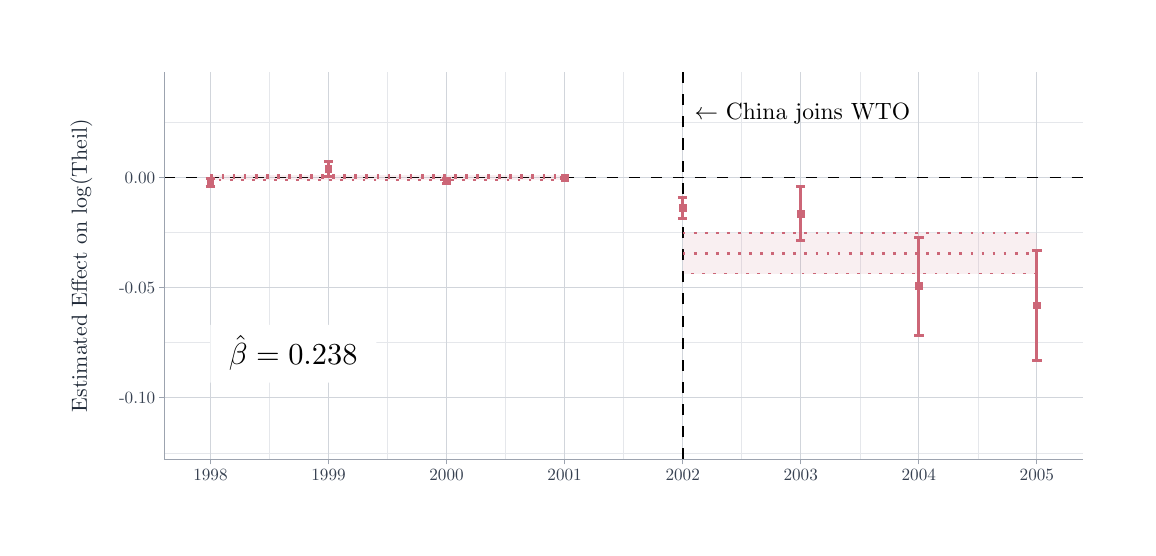
\begin{tikzpicture}[x=1pt,y=1pt]
\definecolor{fillColor}{RGB}{255,255,255}
\path[use as bounding box,fill=fillColor] (0,0) rectangle (397.48,180.67);
\begin{scope}
\path[clip] (  0.00,  0.00) rectangle (397.48,180.67);
\definecolor{drawColor}{RGB}{255,255,255}

\path[draw=drawColor,line width= 0.4pt,line join=round,line cap=round,fill=fillColor] (  0.00,  0.00) rectangle (397.48,180.68);
\end{scope}
\begin{scope}
\path[clip] ( 49.24, 24.64) rectangle (381.48,164.67);
\definecolor{drawColor}{RGB}{255,255,255}
\definecolor{fillColor}{RGB}{255,255,255}

\path[draw=drawColor,line width= 0.4pt,line join=round,line cap=round,fill=fillColor] ( 49.24, 24.64) rectangle (381.48,164.67);
\definecolor{drawColor}{RGB}{229,231,235}

\path[draw=drawColor,line width= 0.2pt,line join=round] ( 49.24, 27.03) --
	(381.48, 27.03);

\path[draw=drawColor,line width= 0.2pt,line join=round] ( 49.24, 66.81) --
	(381.48, 66.81);

\path[draw=drawColor,line width= 0.2pt,line join=round] ( 49.24,106.59) --
	(381.48,106.59);

\path[draw=drawColor,line width= 0.2pt,line join=round] ( 49.24,146.38) --
	(381.48,146.38);

\path[draw=drawColor,line width= 0.2pt,line join=round] ( 87.38, 24.64) --
	( 87.38,164.67);

\path[draw=drawColor,line width= 0.2pt,line join=round] (130.04, 24.64) --
	(130.04,164.67);

\path[draw=drawColor,line width= 0.2pt,line join=round] (172.70, 24.64) --
	(172.70,164.67);

\path[draw=drawColor,line width= 0.2pt,line join=round] (215.36, 24.64) --
	(215.36,164.67);

\path[draw=drawColor,line width= 0.2pt,line join=round] (258.02, 24.64) --
	(258.02,164.67);

\path[draw=drawColor,line width= 0.2pt,line join=round] (300.68, 24.64) --
	(300.68,164.67);

\path[draw=drawColor,line width= 0.2pt,line join=round] (343.35, 24.64) --
	(343.35,164.67);
\definecolor{drawColor}{RGB}{209,213,219}

\path[draw=drawColor,line width= 0.4pt,line join=round] ( 49.24, 46.92) --
	(381.48, 46.92);

\path[draw=drawColor,line width= 0.4pt,line join=round] ( 49.24, 86.70) --
	(381.48, 86.70);

\path[draw=drawColor,line width= 0.4pt,line join=round] ( 49.24,126.48) --
	(381.48,126.48);

\path[draw=drawColor,line width= 0.4pt,line join=round] ( 66.05, 24.64) --
	( 66.05,164.67);

\path[draw=drawColor,line width= 0.4pt,line join=round] (108.71, 24.64) --
	(108.71,164.67);

\path[draw=drawColor,line width= 0.4pt,line join=round] (151.37, 24.64) --
	(151.37,164.67);

\path[draw=drawColor,line width= 0.4pt,line join=round] (194.03, 24.64) --
	(194.03,164.67);

\path[draw=drawColor,line width= 0.4pt,line join=round] (236.69, 24.64) --
	(236.69,164.67);

\path[draw=drawColor,line width= 0.4pt,line join=round] (279.35, 24.64) --
	(279.35,164.67);

\path[draw=drawColor,line width= 0.4pt,line join=round] (322.01, 24.64) --
	(322.01,164.67);

\path[draw=drawColor,line width= 0.4pt,line join=round] (364.68, 24.64) --
	(364.68,164.67);
\definecolor{drawColor}{RGB}{0,0,0}

\path[draw=drawColor,line width= 0.6pt,dash pattern=on 4pt off 4pt ,line join=round] ( 49.24,126.48) -- (381.48,126.48);

\path[draw=drawColor,line width= 0.6pt,dash pattern=on 4pt off 4pt ,line join=round] (236.69, 24.64) -- (236.69,164.67);

\node[text=drawColor,anchor=base west,inner sep=0pt, outer sep=0pt, scale=  0.85] at (240.96,147.41) {$\leftarrow$ China joins WTO};

\path[fill=fillColor] ( 66.05, 52.38) --
	(126.04, 52.38) --
	(126.04, 52.38) --
	(126.04, 52.38) --
	(126.04, 52.38) --
	(126.04, 52.38) --
	(126.04, 52.38) --
	(126.04, 52.38) --
	(126.04, 52.38) --
	(126.04, 52.38) --
	(126.04, 52.38) --
	(126.04, 52.38) --
	(126.04, 52.38) --
	(126.04, 52.38) --
	(126.04, 73.29) --
	(126.04, 73.29) --
	(126.04, 73.29) --
	(126.04, 73.29) --
	(126.04, 73.29) --
	(126.04, 73.29) --
	(126.04, 73.29) --
	(126.04, 73.29) --
	(126.04, 73.29) --
	(126.04, 73.29) --
	(126.04, 73.29) --
	(126.04, 73.29) --
	( 66.05, 73.29) --
	( 66.05, 73.29) --
	( 66.05, 73.29) --
	( 66.05, 73.29) --
	( 66.05, 73.29) --
	( 66.05, 73.29) --
	( 66.05, 73.29) --
	( 66.05, 73.29) --
	( 66.05, 73.29) --
	( 66.05, 73.29) --
	( 66.05, 73.29) --
	( 66.05, 73.29) --
	( 66.05, 73.29) --
	( 66.05, 52.38) --
	( 66.05, 52.38) --
	( 66.05, 52.38) --
	( 66.05, 52.38) --
	( 66.05, 52.38) --
	( 66.05, 52.38) --
	( 66.05, 52.38) --
	( 66.05, 52.38) --
	( 66.05, 52.38) --
	( 66.05, 52.38) --
	( 66.05, 52.38) --
	( 66.05, 52.38) --
	cycle;
\end{scope}
\begin{scope}
\path[clip] ( 49.24, 24.64) rectangle (381.48,164.67);
\definecolor{drawColor}{RGB}{0,0,0}

\node[text=drawColor,anchor=base west,inner sep=0pt, outer sep=0pt, scale=  1.10] at ( 72.69, 59.03) {$\hat{\beta} = 0.238$};
\end{scope}
\begin{scope}
\path[clip] ( 49.24, 24.64) rectangle (381.48,164.67);
\definecolor{drawColor}{RGB}{204,102,119}

\path[draw=drawColor,line width= 1.1pt,line join=round] ( 64.34,126.24) --
	( 67.75,126.24);

\path[draw=drawColor,line width= 1.1pt,line join=round] ( 66.05,126.24) --
	( 66.05,123.25);

\path[draw=drawColor,line width= 1.1pt,line join=round] ( 64.34,123.25) --
	( 67.75,123.25);

\path[draw=drawColor,line width= 1.1pt,line join=round] (107.00,132.33) --
	(110.41,132.33);

\path[draw=drawColor,line width= 1.1pt,line join=round] (108.71,132.33) --
	(108.71,126.93);

\path[draw=drawColor,line width= 1.1pt,line join=round] (107.00,126.93) --
	(110.41,126.93);

\path[draw=drawColor,line width= 1.1pt,line join=round] (149.66,126.32) --
	(153.07,126.32);

\path[draw=drawColor,line width= 1.1pt,line join=round] (151.37,126.32) --
	(151.37,124.31);

\path[draw=drawColor,line width= 1.1pt,line join=round] (149.66,124.31) --
	(153.07,124.31);

\path[draw=drawColor,line width= 1.1pt,line join=round] (192.32,126.45) --
	(195.74,126.45);

\path[draw=drawColor,line width= 1.1pt,line join=round] (194.03,126.45) --
	(194.03,126.04);

\path[draw=drawColor,line width= 1.1pt,line join=round] (192.32,126.04) --
	(195.74,126.04);

\path[draw=drawColor,line width= 1.1pt,line join=round] (234.99,119.33) --
	(238.40,119.33);

\path[draw=drawColor,line width= 1.1pt,line join=round] (236.69,119.33) --
	(236.69,111.55);

\path[draw=drawColor,line width= 1.1pt,line join=round] (234.99,111.55) --
	(238.40,111.55);

\path[draw=drawColor,line width= 1.1pt,line join=round] (277.65,123.35) --
	(281.06,123.35);

\path[draw=drawColor,line width= 1.1pt,line join=round] (279.35,123.35) --
	(279.35,103.65);

\path[draw=drawColor,line width= 1.1pt,line join=round] (277.65,103.65) --
	(281.06,103.65);

\path[draw=drawColor,line width= 1.1pt,line join=round] (320.31,104.91) --
	(323.72,104.91);

\path[draw=drawColor,line width= 1.1pt,line join=round] (322.01,104.91) --
	(322.01, 69.51);

\path[draw=drawColor,line width= 1.1pt,line join=round] (320.31, 69.51) --
	(323.72, 69.51);

\path[draw=drawColor,line width= 1.1pt,line join=round] (362.97,100.10) --
	(366.38,100.10);

\path[draw=drawColor,line width= 1.1pt,line join=round] (364.68,100.10) --
	(364.68, 60.48);

\path[draw=drawColor,line width= 1.1pt,line join=round] (362.97, 60.48) --
	(366.38, 60.48);
\definecolor{fillColor}{RGB}{204,102,119}

\path[fill=fillColor] ( 64.62,123.32) --
	( 67.47,123.32) --
	( 67.47,126.17) --
	( 64.62,126.17) --
	cycle;

\path[fill=fillColor] (107.28,128.20) --
	(110.13,128.20) --
	(110.13,131.05) --
	(107.28,131.05) --
	cycle;

\path[fill=fillColor] (149.94,123.89) --
	(152.80,123.89) --
	(152.80,126.74) --
	(149.94,126.74) --
	cycle;

\path[fill=fillColor] (192.60,124.82) --
	(195.46,124.82) --
	(195.46,127.67) --
	(192.60,127.67) --
	cycle;

\path[fill=fillColor] (235.26,114.01) --
	(238.12,114.01) --
	(238.12,116.87) --
	(235.26,116.87) --
	cycle;

\path[fill=fillColor] (277.93,112.07) --
	(280.78,112.07) --
	(280.78,114.93) --
	(277.93,114.93) --
	cycle;

\path[fill=fillColor] (320.59, 85.78) --
	(323.44, 85.78) --
	(323.44, 88.64) --
	(320.59, 88.64) --
	cycle;

\path[fill=fillColor] (363.25, 78.86) --
	(366.10, 78.86) --
	(366.10, 81.72) --
	(363.25, 81.72) --
	cycle;
\definecolor{fillColor}{RGB}{204,102,119}

\path[fill=fillColor,fill opacity=0.10] (236.69,106.44) --
	(364.68,106.44) --
	(364.68, 91.78) --
	(236.69, 91.78) --
	cycle;

\path[draw=drawColor,line width= 0.6pt,dash pattern=on 1pt off 3pt ,line join=round] (236.69,106.44) --
	(364.68,106.44);

\path[draw=drawColor,line width= 0.6pt,dash pattern=on 1pt off 3pt ,line join=round] (364.68, 91.78) --
	(236.69, 91.78);

\path[fill=fillColor,fill opacity=0.10] ( 66.05,127.32) --
	(194.03,127.32) --
	(194.03,125.65) --
	( 66.05,125.65) --
	cycle;

\path[draw=drawColor,line width= 0.6pt,dash pattern=on 1pt off 3pt ,line join=round] ( 66.05,127.32) --
	(194.03,127.32);

\path[draw=drawColor,line width= 0.6pt,dash pattern=on 1pt off 3pt ,line join=round] (194.03,125.65) --
	( 66.05,125.65);

\path[draw=drawColor,line width= 1.1pt,dash pattern=on 1pt off 3pt ,line join=round] (236.69, 99.11) --
	(364.68, 99.11);

\path[draw=drawColor,line width= 1.1pt,dash pattern=on 1pt off 3pt ,line join=round] ( 66.05,126.48) --
	(194.03,126.48);
\end{scope}
\begin{scope}
\path[clip] (  0.00,  0.00) rectangle (397.48,180.67);
\definecolor{drawColor}{RGB}{156,163,175}

\path[draw=drawColor,line width= 0.3pt,line join=round] ( 49.24, 24.64) --
	( 49.24,164.67);
\end{scope}
\begin{scope}
\path[clip] (  0.00,  0.00) rectangle (397.48,180.67);
\definecolor{drawColor}{RGB}{55,65,81}

\node[text=drawColor,anchor=base east,inner sep=0pt, outer sep=0pt, scale=  0.62] at ( 46.09, 44.78) {-0.10};

\node[text=drawColor,anchor=base east,inner sep=0pt, outer sep=0pt, scale=  0.62] at ( 46.09, 84.56) {-0.05};

\node[text=drawColor,anchor=base east,inner sep=0pt, outer sep=0pt, scale=  0.62] at ( 46.09,124.34) {0.00};
\end{scope}
\begin{scope}
\path[clip] (  0.00,  0.00) rectangle (397.48,180.67);
\definecolor{drawColor}{RGB}{156,163,175}

\path[draw=drawColor,line width= 0.3pt,line join=round] ( 47.49, 46.92) --
	( 49.24, 46.92);

\path[draw=drawColor,line width= 0.3pt,line join=round] ( 47.49, 86.70) --
	( 49.24, 86.70);

\path[draw=drawColor,line width= 0.3pt,line join=round] ( 47.49,126.48) --
	( 49.24,126.48);
\end{scope}
\begin{scope}
\path[clip] (  0.00,  0.00) rectangle (397.48,180.67);
\definecolor{drawColor}{RGB}{156,163,175}

\path[draw=drawColor,line width= 0.3pt,line join=round] ( 49.24, 24.64) --
	(381.48, 24.64);
\end{scope}
\begin{scope}
\path[clip] (  0.00,  0.00) rectangle (397.48,180.67);
\definecolor{drawColor}{RGB}{156,163,175}

\path[draw=drawColor,line width= 0.3pt,line join=round] ( 66.05, 22.89) --
	( 66.05, 24.64);

\path[draw=drawColor,line width= 0.3pt,line join=round] (108.71, 22.89) --
	(108.71, 24.64);

\path[draw=drawColor,line width= 0.3pt,line join=round] (151.37, 22.89) --
	(151.37, 24.64);

\path[draw=drawColor,line width= 0.3pt,line join=round] (194.03, 22.89) --
	(194.03, 24.64);

\path[draw=drawColor,line width= 0.3pt,line join=round] (236.69, 22.89) --
	(236.69, 24.64);

\path[draw=drawColor,line width= 0.3pt,line join=round] (279.35, 22.89) --
	(279.35, 24.64);

\path[draw=drawColor,line width= 0.3pt,line join=round] (322.01, 22.89) --
	(322.01, 24.64);

\path[draw=drawColor,line width= 0.3pt,line join=round] (364.68, 22.89) --
	(364.68, 24.64);
\end{scope}
\begin{scope}
\path[clip] (  0.00,  0.00) rectangle (397.48,180.67);
\definecolor{drawColor}{RGB}{55,65,81}

\node[text=drawColor,anchor=base,inner sep=0pt, outer sep=0pt, scale=  0.62] at ( 66.05, 17.21) {1998};

\node[text=drawColor,anchor=base,inner sep=0pt, outer sep=0pt, scale=  0.62] at (108.71, 17.21) {1999};

\node[text=drawColor,anchor=base,inner sep=0pt, outer sep=0pt, scale=  0.62] at (151.37, 17.21) {2000};

\node[text=drawColor,anchor=base,inner sep=0pt, outer sep=0pt, scale=  0.62] at (194.03, 17.21) {2001};

\node[text=drawColor,anchor=base,inner sep=0pt, outer sep=0pt, scale=  0.62] at (236.69, 17.21) {2002};

\node[text=drawColor,anchor=base,inner sep=0pt, outer sep=0pt, scale=  0.62] at (279.35, 17.21) {2003};

\node[text=drawColor,anchor=base,inner sep=0pt, outer sep=0pt, scale=  0.62] at (322.01, 17.21) {2004};

\node[text=drawColor,anchor=base,inner sep=0pt, outer sep=0pt, scale=  0.62] at (364.68, 17.21) {2005};
\end{scope}
\begin{scope}
\path[clip] (  0.00,  0.00) rectangle (397.48,180.67);
\definecolor{drawColor}{RGB}{31,41,55}

\node[text=drawColor,rotate= 90.00,anchor=base,inner sep=0pt, outer sep=0pt, scale=  0.79] at ( 21.42, 94.66) {Estimated Effect on $\log($Theil$)$};
\end{scope}
\end{tikzpicture}
